\chapter{Strumenti numerici indicatori - parte VI}

\begin{figure}[h]
    \centering
    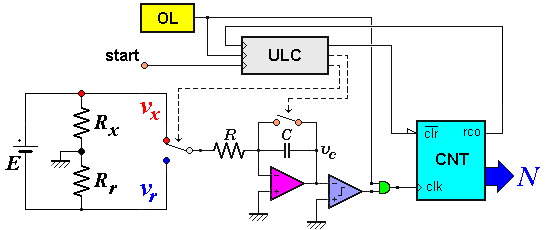
\includegraphics[scale = 1.5]{Architettura dell'ohmetro.png}
\end{figure}

\newpage    

\section{Dal voltmetro all'amperometro per DC}
\footnote{Slide della prof | SDME 4 Strumenti numerici indicatori - parte VI | pag 3 \\  
Appunti | 2025-05-13 | pag 2 - 3 | 2025-06-23 Ricevimento | pag 9, 11}

L'obbiettivo di questo capitolo è quello di costruire un'architettura per un amperometro, 
partendo dall'architettura di un voltmetro e sfruttando la legge di Ohm. \newline 

Ritornando all'architettura del voltmetro, possiamo dividerla in due parti:

\begin{figure}[h]
    \centering
    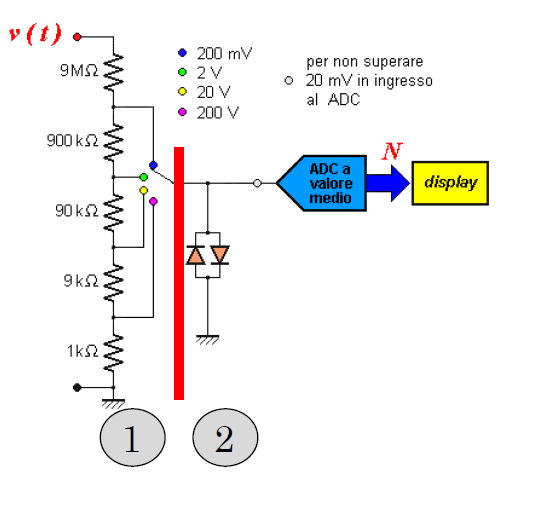
\includegraphics[scale = 1]{Divisione degli stadi di un'architettura di un voltmetro.PNG}
\end{figure}

La parte a sinistra, scritta con il numero 1, viene definita come stadio d'ingresso di un voltmetro. \newline 

La parte a destra, scritta con il numero 2, viene definita come circuito digitale. \newline 

Dalla legge di Ohm, sappiamo che la corrente i dipende v e da R come:

{
    \Large 
    \begin{equation}
        \begin{split}
            v &= R \cdot i
            \\
            &\updownarrow
            \\
            i &= \frac{v}{R} 
        \end{split}
    \end{equation}
}

\newpage 

Sapendo che la corrente verrà determinata in modo indiretta utilizzando questa relazione, 
possiamo cambiare lo stadio di ingresso del voltmetro e adattarlo come amperometro: 

\begin{figure}[h]
    \centering
    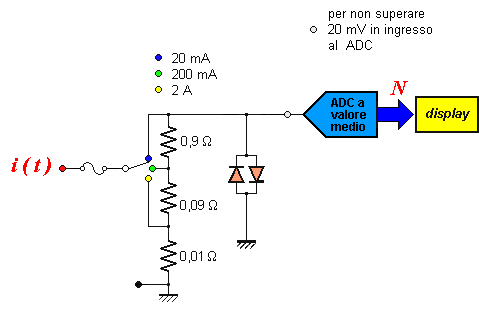
\includegraphics[scale = 1.5]{Architettura di un amperometro.png}
\end{figure}

Lo stadio di ingresso, partendo dalla boccola calda dello strumento di misura (pallino rosso nel circuito), 
prima della rete resistiva, è presente un fusibile. \newline 

Il fusibile è una resistenza di valore idealmente nullo, nella realtà avrà un valore nominale molto basso, 
che ha la proprietà di bruciarsi in caso ci sia una corrente molto elevata nel ramo. \newline 

Nell'architettura dell'amperometro viene posizionato un fusibile nello stadio di ingresso dello strumento per proteggere la rete resistiva, ma in particolare l'ADC a valor medio, 
da tensione e/o correnti molto elevate. \newline 

In caso di malfunzionamento, il fusibile si brucia e va immediatamente sostituito. \newline 

Notando il selettore delle portate, in questo tipo di architetture le portate passano da 4 a 3. \newline 

Se il selettore è posizionato in una portata diversa da quella di 20 mA (pallino blu), 
ci sono dei resistori (o resistore) che non sono percorsi dalla corrente i(t), 
e quindi non avranno una caduta di tensione nel nodo in comune con l'ADC a valor medio. \newline 

Rispetto al valore standard della rete resistiva dei voltmetri di 10 $M \Omega$, 
in questo caso, la rete resistiva ha resistenza pari a 1 $\Omega$, perchè, nell'amperometro ideale, la sua resistenza dovrebbe essere nulla. \newline 

Siccome complessivamente la rete resistiva deve massimo generare 20 mV di tensione per proteggere l'ADC, 
la corrente massima che può circolare nell'amperometro è di: 

{
    \Large
    \begin{equation}
        \begin{split}
            i_{max} &= \frac{v_{max}}{R}
            \\
            &= \frac{20 \text{ }[mV]}{0.01 \text{ }[\Omega]}
            \\
            &= 
            2 \text{ } [A]
        \end{split}
    \end{equation}
}

Si prende la R minima perchè passerà una corrente maggiore nel circuito. \newline 

Ultima considerazione da svolgere riguardo l'architettura sotto un punto di vista metrologico: 
non è possibile quantificare la resistenza del fusibile perchè essa varia in base alla corrente di ingresso e ciò porterà dei problemi nel calcolo della tensione per l'ADC. \newline 

\newpage 

\section{Schemi per il convertitore i-v}
\footnote{Slide della prof | SDME 4 Strumenti numerici indicatori - parte VI | pag 4 - 7 \\  
Appunti | 2025-05-13 | pag 3 - 8}

Idealmente, il convertitore corrente-tensione è il seguente: 

\begin{figure}[h]
    \centering
    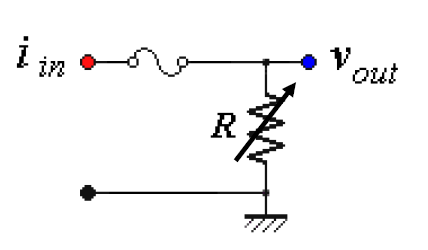
\includegraphics[scale = 1]{Convertitore corrente tensione ideale.png}
\end{figure}

dove R è una resistenza variabile che cambia in base alla portata dell'amperometro scelta. \newline 

Dal punto di vista metrologico, è meglio posizionare il fusibile prima o dopo la resistenza variabile? \newline 

Per misurare la corrente in un circuito reale, avremo il seguente schema: 

\begin{figure}[h]
    \centering
    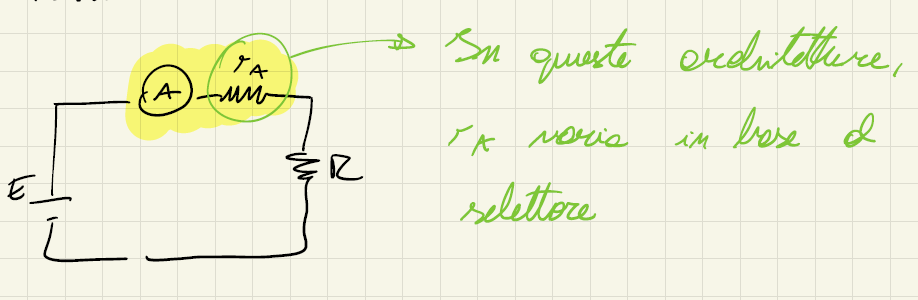
\includegraphics[scale = 0.8]{Circuito di misura della corrente in un circuito reale con annotazioni.PNG}
\end{figure}

Come scritto nelle note, $r_A$, cioè la resistenza dell'amperometro varia in base alla portata dell'amperometro stesso, 
e, in un circuito ideale, $r_A$ è nulla. \newline 

Quindi, ritornando al convertitore corrente-tensione, il convertitore deve avere una resistenza che tende a zero con l'aumentare della portata. \newline 

Confrontando le seguenti architetture: 

\begin{figure}[h]
    \centering
    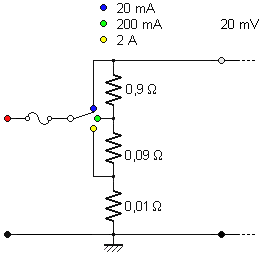
\includegraphics[scale = 1]{Stadio di ingresso amperometro A.png}
    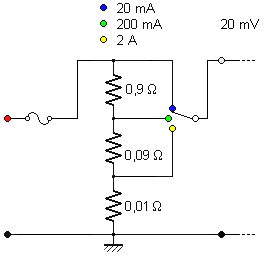
\includegraphics[scale = 1]{Stadio di ingresso amperometro B.png}
\end{figure}

dove, la figura a sinistra viene chiamata architettura (A), la figura a destra viene chiamata architettura (B). \newline 

\newpage 

Calcoliamo la resistenza dell'amperometro $r_A$ in base alla portata scelta: 

\begin{figure}[h]
    \centering
    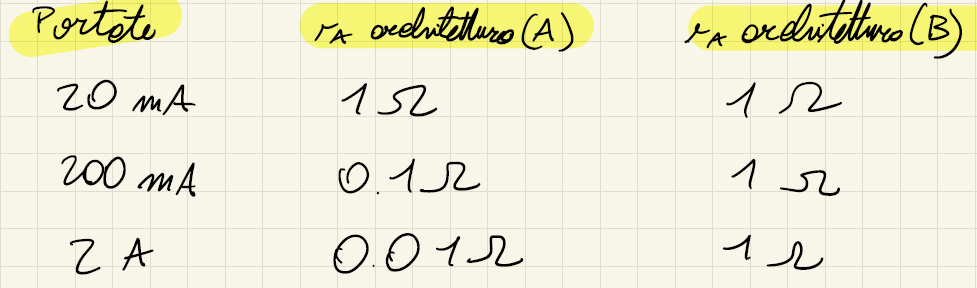
\includegraphics[scale = 0.8]{Portate amperometri e confronti con due tipi di architetture.PNG}
\end{figure}

Dalla seguente tabella si nota che, all'aumentare della portata, la resistenza $r_A$ diminuisce nell'architettura (A), 
ed ecco perchè è uno tra i motivi per cui è stato scelto questo tipo di architettura rispetto alle (B). \newline 

La resistenza $r_A$, nell'architettura (B), rimane costante perchè la corrente sotto misura percorre sempre tutti i resistori, anche se la portata dell'amperometro varia. \newline 

Un altro motivo per cui si sceglie l'architettura (A) rispetto alla (B) è dovuto all'effetto Joule sui resistori. \newline 

Nell'architettura (B) si dissipa più energia rispetto all'architettura (A). \newline 

Dall'elettrotecnica, sappiamo che la potenza P dissipata su un resistore si può esprimere come:

{
    \Large 
    \begin{equation}
        \begin{split}
            P &= v \cdot i 
            \\ 
            &= (R \cdot i) \cdot i 
            \\
            &= R \cdot i^{2}   
        \end{split}
    \end{equation}
}

Consideriamo l'architettura (A) e la portata di 20 mA:

{
    \Large
    \begin{equation}
        \begin{split}
            P &= R \cdot i^{2}
            \\
            &= 1 \text{ }[\Omega] \cdot (20 \text{ } [mA])^{2}
            \\
            &= 
            0.4 \text{ }[mW] 
        \end{split}
    \end{equation}
}

Sui singoli resistori è dissipata la seguente potenza: 

\begin{figure}[h]
    \centering
    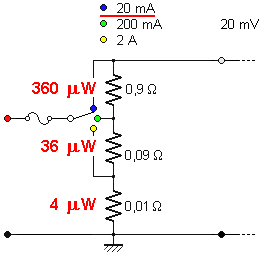
\includegraphics[scale = 0.8]{Potenza dissipata in un amperometro con 20mA.png}
\end{figure}

Consideriamo l'architettura (A) e la portata di 200 mA:

{
    \Large
    \begin{equation}
        \begin{split}
            P &= R \cdot i^{2}
            \\
            &= 0.1 \text{ }[\Omega] \cdot (200 \text{ } [mA])^{2}
            \\
            &= 
            4 \text{ }[mW] 
        \end{split}
    \end{equation}
}

\newpage 

Sui singoli resistori è dissipata la seguente potenza: 

\begin{figure}[h]
    \centering
    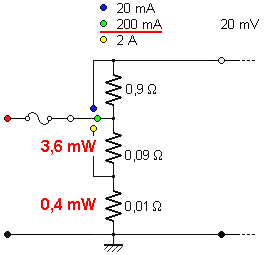
\includegraphics[scale = 0.8]{Potenza dissipata in un amperometro con 200mA.png}
\end{figure}

Consideriamo l'architettura (A) e la portata di 2 A:

{
    \Large
    \begin{equation}
        \begin{split}
            P &= R \cdot i^{2}
            \\
            &= 1 \text{ }[m\Omega] \cdot (2 \text{ } [A])^{2}
            \\
            &= 
            40 \text{ }[mW] 
        \end{split}
    \end{equation}
}

Sui singoli resistori è dissipata la seguente potenza: 

\begin{figure}[h]
    \centering
    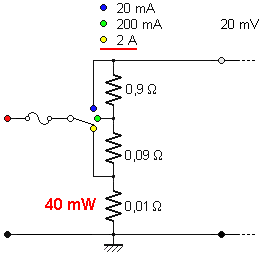
\includegraphics[scale = 0.8]{Potenza dissipata in un amperometro con 2A.png}
\end{figure}

Consideriamo l'architettura (B) e la portata di 20 mA:

{
    \Large
    \begin{equation}
        \begin{split}
            P &= R \cdot i^{2}
            \\
            &= 1 \text{ }[\Omega] \cdot (20 \text{ } [mA])^{2}
            \\
            &= 
            0.4 \text{ }[mW] 
        \end{split}
    \end{equation}
}

Consideriamo l'architettura (B) e la portata di 200 mA:

{
    \Large
    \begin{equation}
        \begin{split}
            P &= R \cdot i^{2}
            \\
            &= 1 \text{ }[\Omega] \cdot (200 \text{ } [mA])^{2}
            \\
            &= 
            40 \text{ }[mW] 
        \end{split}
    \end{equation}
}

Consideriamo l'architettura (B) e la portata di 2 A:

{
    \Large
    \begin{equation}
        \begin{split}
            P &= R \cdot i^{2}
            \\
            &= 1 \text{ }[\Omega] \cdot (2 \text{ } [A])^{2}
            \\
            &= 
            4 \text{ }[W] 
        \end{split}
    \end{equation}
}

Nell'architettura (A), dalla portata più piccola alla portata più grande, si dissipano due ordini di grandezza: 
si passa dai 0.4 mW dei 20 mA ai 40 mW dei 2 A. \newline 

A differenza dell'architettura (B) che, dalla portata più piccola alla portata più grande, si dissipano  quattro ordini di grandezza: 
si passa dai 0.4 mW dei 20 mA ai 4 W dei 2 A. \newline 

4 W da dissipare sono tanti per uno strumento, come un tester, che non ha una ventola. \newline 

Anche per questo motivo è meglio l'architettura (A) perchè, dal punto di vista energetico, è più efficiente e, all'aumentare della portata, 
dissipa meno energia rispetto l'architettura (B). \newline 

Una regola che possiamo tratte da questi calcoli è che 
più è alta la potenza da smaltire, 
più deve essere grande fisicamente lo strumento, quindi, se possibile, meglio efficientare il processo di misura. \newline 

\newpage 

\section{L'amperometro per DC e AC}
\footnote{Slide della prof | SDME 4 Strumenti numerici indicatori - parte VI | pag 8 \\  
Appunti | 2025-05-13 | pag 9 | 2025-06-23 Ricevimento | pag 9, 11}

Un esempio di architettura di amperometro per DC e AC è la seguente: 

\begin{figure}[h]
    \centering
    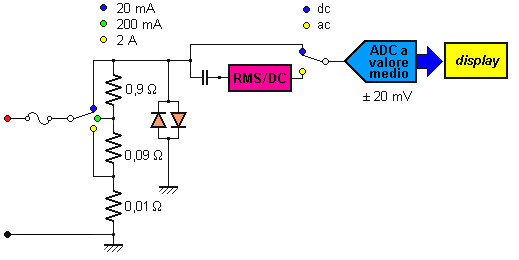
\includegraphics[scale = 1.5]{Amperometro per AC e DC.png}
\end{figure}

Si può posizionare nell'architettura al posto del blocco RMS/DC un blocco TRMS/DC: 
dipende sempre se lo strumento di cui si fa l'architettura ne è provvisto. \newline 

L'architettura dell'amperometro DC/AC è la stessa del voltmetro DC/AC, 
ma lo stadio di ingresso è diverso. \newline 

I resistori della rete resistiva sono resistori di shunt perchè sono resistori che mantengono il loro valore di resistenza vicino a quello nominale e lo mantengono in modo stabile. \newline

Dopo lo stadio di ingresso, anche nell'amperometro si possono fare le stesse conclusioni e osservazioni del voltmetro DC/AC. \newline 

La tensione che va all'ADC non è calcolata in base ad un rapporto con la tensione di ingresso, 
bensì, grazie alla legge di ohm, è calcolata come un prodotto tra la corrente di ingresso ed i resistori in cui si ha una caduta di tensione. \newline 

\newpage 

\subsection{L'amperometro e la perturbazione}
\footnote{Slide della prof | SDME 4 Strumenti numerici indicatori - parte VI | pag 9 - 10 \\  
Appunti | 2025-05-13 | pag 9 - 10}

Come scritto più volte in queste pagine, purtroppo svolgere una misura comporta una perturbazione rispetto al circuito da misurare. \newline 

Dato il circuito ideale: 

\begin{figure}[h]
    \centering
    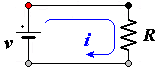
\includegraphics[scale = 2]{corrente in un circuito semplice.png}
\end{figure}

Idealmente, se si volesse misurare la corrente, basterebbe posizionare un amperometro: 

\begin{figure}[h]
    \centering
    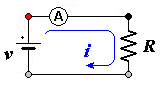
\includegraphics[scale = 2]{misura ideale della corrente in un circuito semplice.png}
\end{figure}

Ma nella realtà, l'amperometro presenterà una resistenza interna $r_A$:

\begin{figure}[h]
    \centering
    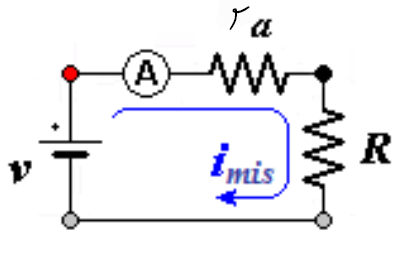
\includegraphics[scale = 0.9]{misura reale della corrente in un circuito semplice.png}
\end{figure}

che perturberà, e quindi cambierà, la corrente nel circuito. \newline 

Dalla legge di Ohm, sappiamo che il valore della corrente nel circuito ideale è:

{
    \Large 
    \begin{equation}
        i = \frac{v}{R}
    \end{equation}
}

Invece, nel circuito reale, essendo $r_A$ in serie con R, la corrente misurata sarà:

{
    \Large 
    \begin{equation}
        i_{mis} = \frac{v}{R + r_A}
    \end{equation}
}


Quindi, considerando che i valori dei resistori sono positivi e la tensione la consideriamo anche essa positiva, 
avremo questa relazione tra i e $i_{mis}$: 

{
    \Large 
    \begin{equation}
        i < i_{mis}
    \end{equation}
}

Inoltre, la perturbazione di i rispetto a $i_{mis}$ vale:

{
    \Large
    \begin{equation}
        \frac{\delta i}{i}
        = 
        -
        \frac{r_A}{r_A + R}
    \end{equation}
}

Dalla formula di $\frac{\delta i}{i}$, non solo $i_{mis}$ è minore, ma è anche una sottostima di i perchè la perturbazione è di segno negativo. \newline 

Per quanto riguarda l'architettura dell'amperometro AC/DC: 

\begin{figure}[h]
    \centering
    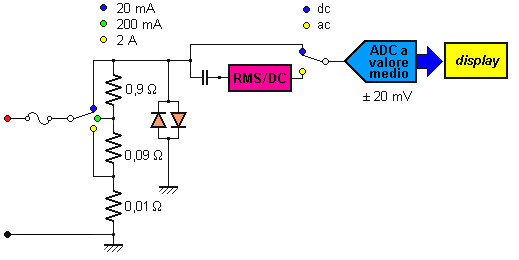
\includegraphics[scale = 1.5]{Amperometro per AC e DC.png}
\end{figure}

è difficile determinare e calcolare a priori la $r_A$ dell'amperometro perchè, ad esempio, 
il fusibile e il commutatore possono avere un valore nominale  di qualche decina di $m \Omega$. \newline 

Sommate le resistenze parassite, 
queste ultime possono essere paragonabili alla rete resistiva degli shunt. \newline 

Siccome non è possibile quantificare il valore di $r_A$ a priori, per avere una perturbazione bassa della corrente, 
cioè far tendere a zero $\frac{\delta i}{i}$, 
quando si fa una misura della corrente reale con un amperometro reale, 
bisogna mettere in serie all'amperometro un resistore che sia di diversi ordini di grandezza più grande di $r_A$. \newline 

In formule:

{
    \Large
    \begin{equation}
            \frac{\delta i}{i} \to 0 \text{ se } R >> r_A
    \end{equation}
}

La correzione in tensione è sempre più facile che una correzione fatta in corrente. \newline 

Non potendo correggere con precisione la perturbazione della misura dell'amperometro, 
è preferibile fare misure di tensione invece che di corrente. \newline

\newpage 

\section{Voltmetro + Amperometro}
\footnote{Slide della prof | SDME 4 Strumenti numerici indicatori - parte VI | pag 11 - 13 \\  
Appunti | 2025-05-13 | pag 10}

Sapendo che lo stadio di elaborazione è lo stesso, 
si possono unire le architetture dell'amperometro e del voltmetro con questo tipo di architettura: 

\begin{figure}[h]
    \centering
    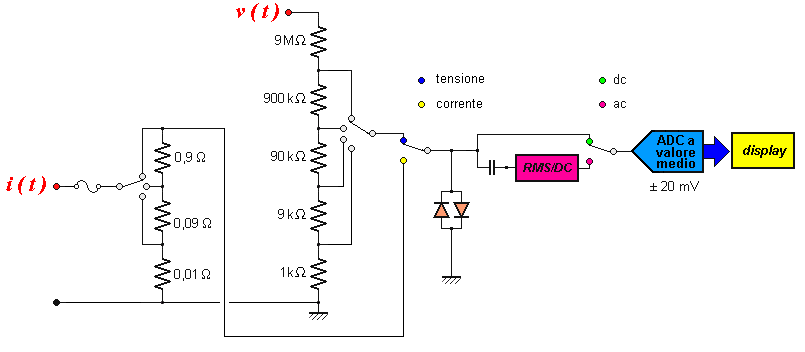
\includegraphics[scale = 0.8]{Amperometro + Voltmetro.png}
\end{figure}

Dato un multimetro come il seguente: 

\begin{figure}[h]
    \centering
    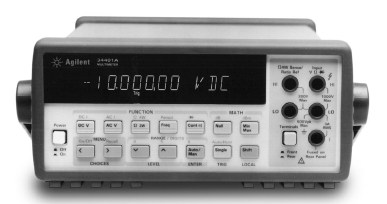
\includegraphics[scale = 1]{multimetro da banco.png}
\end{figure}

Il corrispettivo tra boccole dello strumento e l'architettura è la seguente: 

\begin{figure}[h]
    \centering
    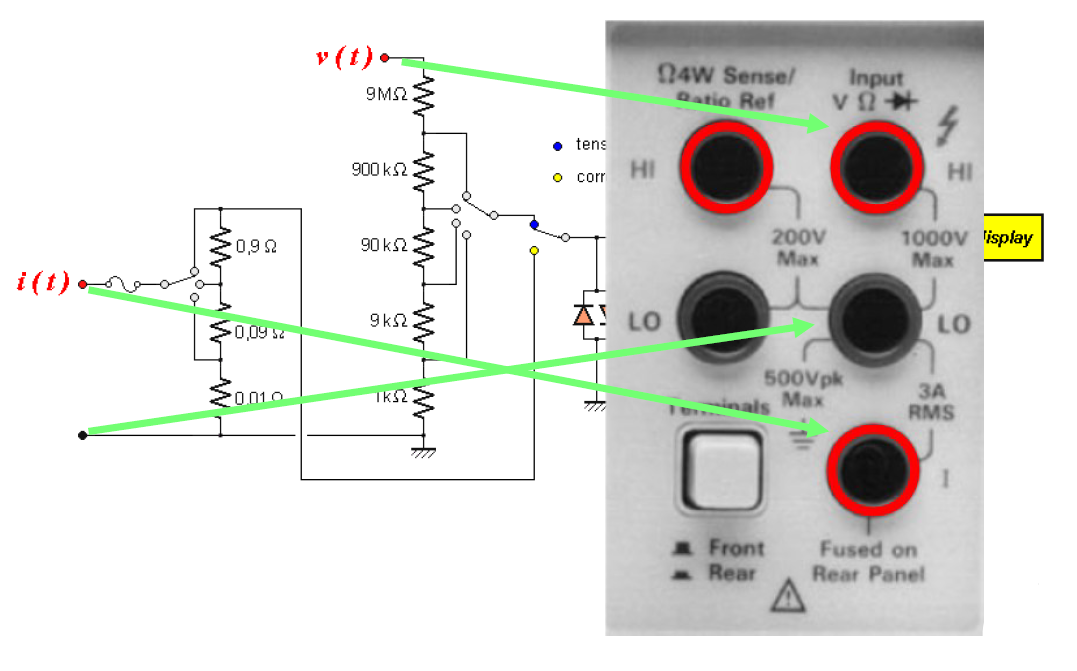
\includegraphics[scale = 0.7]{Boccole Amperometro + Voltmetro reale.png}
\end{figure}

Dalla figura delle boccole, si può notare la scritta "Fused on Rear Panel"; 
come scritto precedentemente, il costruttore del multimetro indica sullo strumento dove si trova il fusibile, 
in modo da individuarlo e sostituirlo facilmente in caso di guasto. \newline 

\newpage 

Per quanto riguarda i selettori, nel multimetro reale possono essere cambiati con i seguenti pulsanti: 

\begin{figure}[h]
    \centering
    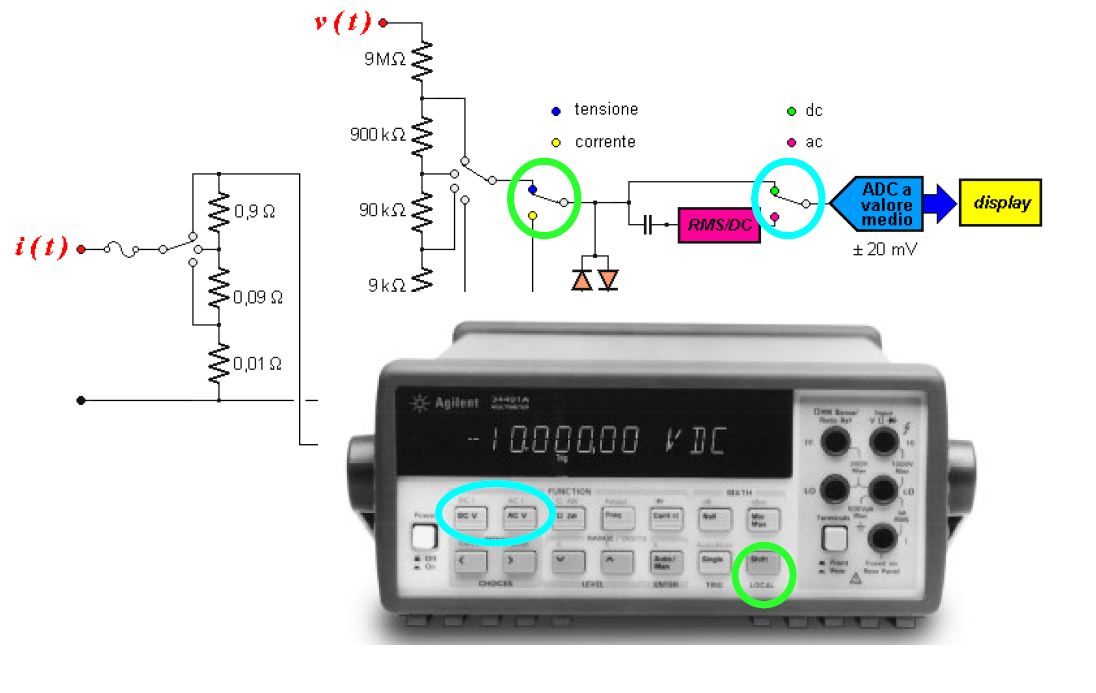
\includegraphics[scale = 0.7]{Selettori Amperometro + Voltmetro reale.png}
\end{figure}

\newpage 

\section{Dal voltmetro all'ohmmetro}
\footnote{Slide della prof | SDME 4 Strumenti numerici indicatori - parte VI | pag 14 - 15 \\  
Appunti | 2025-05-13 | pag 10 - 11 }

Sapendo il principio di funzionamento dell'architettura dell'AD a valor medio tensione - tempo doppia rampa studiata nel voltmetro: 

\begin{figure}[h]
    \centering
    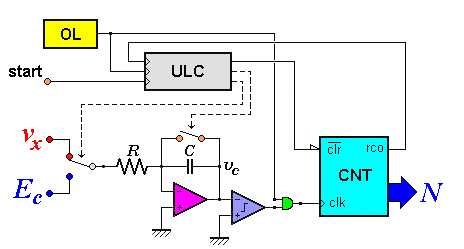
\includegraphics[scale = 1]{convertitore AD a valor medio tensione - tempo a doppia rampa.PNG}
\end{figure}

e che la tensione misurata media $\overline{v_x}$ nell'intervallo $[t_0, t_1]$ vale: 

{
    \Large
    \begin{equation}
        \left.
        \overline{v_x}
        \right|_{[t_0, t_1]}
        = 
        \frac{- E_c }{N_{max}} N
    \end{equation}
}

Possiamo modificare un pochino l'architettura per adattarla ad un ohmmetro, quindi ad una architettura che misura la resistenza di un bipolo $R_x$: 

\begin{figure}[h]
    \centering
    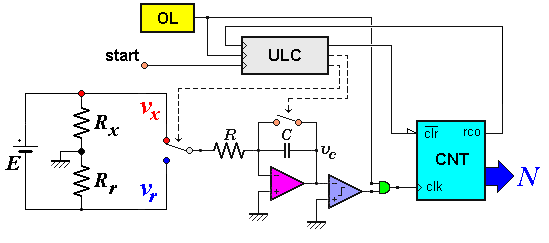
\includegraphics[scale = 1.5]{Architettura ohmetro.png}
\end{figure}

$R_x$, con questo tipo di architettura, equivale a: 

{
    \Large
    \begin{equation}
        R_x 
        = 
        \frac{R_r}{N_{max}} N
    \end{equation}
}

Rispetto al voltmetro, sono presenti dei componenti in più: un riferimento di f.e.m. E e un partitore di tensione tra $R_x$ e $R_r$, 
dove $R_r$ è una resistenza di riferimento e che quindi deve avere un valore noto stabile. \newline 

Come il voltmetro, $v_r$ è minore di zero, invece $v_x$ è maggiore di zero. \newline 

\newpage 

\subsection{Analisi funzionamento ideale}
\footnote{Slide della prof | SDME 4 Strumenti numerici indicatori - parte VI | pag 16 - 17 \\  
No Appunti }

Come nel voltmetro, le tensioni nel tempo sono le seguenti: 

\begin{figure}[h]
    \centering
    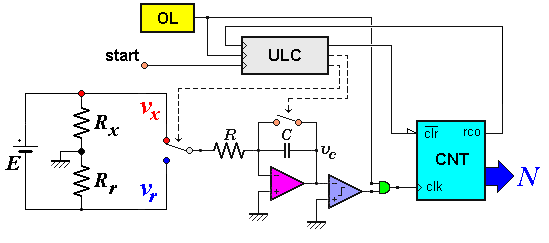
\includegraphics[scale = 1.5]{Architettura ohmetro.png}
    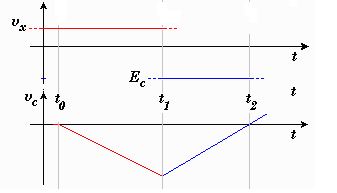
\includegraphics[scale = 1.5]{Andamento di vx e vc in un ADC a valor medio.png}
\end{figure}

(Nella figura $E_c$ è uguale a $v_r$ nell'architettura dell'ohmmetro) \newline 

Le tensioni vengono ricavate con le seguenti operazioni matematiche: 

{
    \Large 
    \begin{equation}
        \begin{cases}
            v_c (t_0) = 0
            \\
            v_c (t_1) = v_c (t_0) + \int_{t_0}^{t_1} \frac{v_x (t)}{- RC} dt 
            \\
            v_c (t_2) = v_c (t_1) + \int_{t_1}^{t_2} \frac{v_r (t)}{- RC} dt
            \\ 
            v_c (t_2) = 0
        \end{cases}
    \end{equation}
}

Sostituendo i valori noti e facendo dei semplici passi algebrici, 
$v_c (t_2)$ diventa: 

{
    \Large 
    \begin{equation}
        \begin{split}
            v_c (t_2) &= v_c (t_1) + \int_{t_1}^{t_2} \frac{v_r (t)}{- RC} dt
            \\
            & = v_c (t_0) + \int_{t_0}^{t_1} \frac{v_x (t)}{- RC} dt + \int_{t_1}^{t_2} \frac{v_r (t)}{- RC} dt
            \\
            &\downarrow
            \\
            0 &= 0 + \int_{t_0}^{t_1} \frac{v_x (t)}{- RC} dt + \int_{t_1}^{t_2} \frac{v_r (t)}{- RC} dt
            \\
            - \int_{t_0}^{t_1} \frac{v_x (t)}{- RC} dt 
            &=
            \int_{t_1}^{t_2} \frac{v_r (t)}{- RC} dt
            \\
            \int_{t_0}^{t_1} \frac{v_x (t)}{RC} dt 
            &=
        \end{split}
    \end{equation}
}

Quindi alla fine, come il caso del voltmetro, bisogna valutare la stabilità dell'equazione: 

{
    \Large 
    \begin{equation}
       \int_{t_0}^{t_1} \frac{v_x (t)}{RC} dt 
            = 
        \int_{t_1}^{t_2} \frac{v_r (t)}{- RC} dt  
    \end{equation}
}

\newpage 

\subsection{Primo vincolo sulla stabilità}
\footnote{Slide della prof | SDME 4 Strumenti numerici indicatori - parte VI | pag 18 \\  
No Appunti }

Come il caso del voltmetro, dobbiamo valutare il primo vincolo sulla stabilità dei parametri che compongono l'equazione nel periodo $[t_0, t_2]$: 

{
    \Large 
    \begin{equation}
       \int_{t_0}^{t_1} \frac{v_x (t)}{RC} dt 
            = 
        \int_{t_1}^{t_2} \frac{v_r (t)}{- RC} dt  
    \end{equation}
}

$R \cdot C$ è un parametro costante nell'intervallo $[t_0, t_2]$, 
quindi possiamo mandare fuori dall'integrale in entrambi i membri dell'equazione, e con diversi passi algebrici, 
l'equazione diventa: 

{
    \Large 
    \begin{equation}
        \begin{split}
            \int_{t_0}^{t_1} \frac{v_x (t)}{RC} dt 
            &= 
        \int_{t_1}^{t_2} \frac{v_r (t)}{- RC} dt 
        \\
        \frac{1}{RC}
        \int_{t_0}^{t_1} v_x (t) dt 
        &= 
        - \frac{1}{RC}
        \int_{t_1}^{t_2} v_r (t) dt
        \\
        \int_{t_0}^{t_1} v_x (t) dt 
        &= 
        - 
        \int_{t_1}^{t_2} v_r (t) dt
        \end{split}
    \end{equation}
}

Quindi alla fine dovremo valutare la stabilità di $v_x (t)$ e $v_r (t)$ nel periodo $[t_0, t_2]$ nell'equazione: 

{
    \Large 
    \begin{equation}
       \int_{t_0}^{t_1} v_x (t) dt 
        = 
        - 
        \int_{t_1}^{t_2} v_r (t) dt 
    \end{equation}
}

\newpage 

\subsection{Il convertitore R - v}
\footnote{Slide della prof | SDME 4 Strumenti numerici indicatori - parte VI | pag 19 \\  
No Appunti }

Sapendo che nell'ohmmetro le tensioni di $v_x (t)$ e $v_r (t)$ sono ricavate da questo circuito: 

\begin{figure}[h]
    \centering
    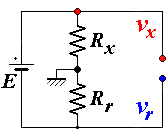
\includegraphics[scale = 1.5]{Partitore di tensione di riferimento nell'ohmetro.png}
\end{figure}

Risolvendo questo semplice problema di elettrotecnica, avremo che $v_x(t)$ e $v_r (t)$ sono esprimibili come:

{
    \Large 
    \begin{equation}
        \begin{cases}
            v_x (t) = E \cdot \frac{R_x}{R_x + R_r} (t)
            \\
            v_r (t) = - E \cdot \frac{R_r}{R_x + R_r} (t)
        \end{cases}
    \end{equation}
}

\begin{tcolorbox}
Per adesso scriviamo che $v_x$ e $v_r$ sono funzioni che variano nel tempo (ma poi vedremo come semplificare i conti)
\end{tcolorbox} 

Quindi, possiamo esprimere l'equazione dopo il primo vincolo sulla stabilità: 

{
    \Large 
    \begin{equation}
        \begin{split}
        \int_{t_0}^{t_1} v_x (t) dt 
        &= 
        - 
        \int_{t_1}^{t_2} v_r (t) dt   
        \\
        &\downarrow
        \\
        \int_{t_0}^{t_1} 
        E \cdot \frac{R_x}{R_x + R_r} (t)
        dt 
        &= 
        - 
        \int_{t_1}^{t_2} 
        - E \cdot \frac{R_r}{R_x + R_r} (t)
        dt  
        \end{split}
    \end{equation}
}

\newpage 

\subsection{Secondo vincolo sulla stabilità}
\footnote{Slide della prof | SDME 4 Strumenti numerici indicatori - parte VI | pag 20 \\  
No Appunti }

Dopo il primo vincolo sulla stabilità, e aver espresso le tensioni $v_x (t)$ e $v_r (t)$ in funzione di E, $R_r$ e $R_x$: 

{
    \Large 
    \begin{equation}
        \int_{t_0}^{t_1} 
        E \cdot \frac{R_x}{R_x + R_r} (t)
        dt 
        = 
        - 
        \int_{t_1}^{t_2} 
        - E \cdot \frac{R_r}{R_x + R_r} (t)
        dt  
    \end{equation}
}

dobbiamo valutare se questi componenti sono stabili nel periodo $[t_0, t_2]$. \newline 

Se E, $R_x$ e $R_r$ sono costanti lungo il periodo $[t_0, t_2]$, 
la funzione non dipende più dal tempo t, 
quindi, con diversi passaggi algebrici,
diventa:

{
    \Large 
    \begin{equation}
        \begin{split}
        \int_{t_0}^{t_1} 
        E \cdot \frac{R_x}{R_x + R_r} (t)
        dt 
        &= 
        - 
        \int_{t_1}^{t_2} 
        - E \cdot \frac{R_r}{R_x + R_r} (t)
        dt
        \\
        &\downarrow
        \\
        \int_{t_0}^{t_1} 
        E \cdot \frac{R_x}{R_x + R_r}
        dt 
        &= 
        - 
        \int_{t_1}^{t_2} 
        - E \cdot \frac{R_r}{R_x + R_r}
        dt
        \\
        E \cdot \frac{R_x}{R_x + R_r}
        \int_{t_0}^{t_1} 
        dt 
        &= 
        E \cdot \frac{R_r}{R_x + R_r}
        \int_{t_1}^{t_2} 
        dt
        \\
        R_x
        \int_{t_0}^{t_1} 
        dt 
        &= 
        R_r
        \int_{t_1}^{t_2} 
        dt
        \\
        R_x (t_1 - t_0)
        &= 
        R_r (t_2 - t_1)
        \end{split}  
    \end{equation}
}

\newpage 

\subsection{Espressione finale}
\footnote{Slide della prof | SDME 4 Strumenti numerici indicatori - parte VI | pag 21 \\  
Appunti | 2025-06-23 Ricevimento | pag 9, 11}


Sapendo che, il principio di funzionamento dell'architettura dell'ohmetro è come quella del voltmetro, 
e che quindi è presente anche un OL-GATE-CNT, 
i periodi $[t_0, t_1]$ e $[t_1, t_2]$ possono espressi come: 

{
    \Large 
    \begin{equation}
        \begin{cases}
            t_1 - t_0 = N_{max} \cdot \tau 
            \\
            t_2 - t_1 = N \cdot \tau
        \end{cases}
    \end{equation}
}

dove $N_{max}$ è la capienza massima del CNT e $\tau$ è il tempo di un clock dell'OL. \newline 

Sostituendo questi valori all'equazione dopo il secondo vincolo sulla stabilità e con dei semplici passaggi algebrici: 

{
    \Large 
    \begin{equation}
        \begin{split}
        R_x (t_1 - t_0)
        &= 
        R_r (t_2 - t_1)   
        \\ 
        &\downarrow
        \\
        R_x \cdot [N_{max} \cdot \tau ]
        &\approx 
        R_r \cdot [N \cdot \tau]
        \\
        R_x 
        &\approx 
        R_r \cdot \frac{N \cdot \tau}{N_{max} \cdot \tau}
        \end{split}
    \end{equation}
}

Prima di semplificare il $\tau$ nel rapporto di $R_x$, 
facciamo una piccola osservazione. \newline 

Rispetto al voltmetro, nell'ohmetro l'OL Oscillatore Locale non deve per forza essere un OL veloce quarzato 
perchè basta che la stabilità di $\tau$ sia garantita nel periodo $[t_0, t_2]$, 
periodo che sarà molto lungo e sarà di qualche frazione di secondo. \newline

Nell'ohmmetro, l'OL può essere realizzato, al posto del quarzo, con una rete RC e un OpAmp. \newline 

L'intervallo $[t_0, t_2]$, minore di 200 ms, permette di considerare stabili e costanti i valori di RC nell'OL 
con rete RC e un OpAmp. \newline 

Nell'intervallo di tempo $[t_0, t_2]$ si considera RC costanti anche nell'OL. \newline 

Ora continuiamo le semplificazioni. \newline 

Visto che $\tau$ è lo stesso perchè gli intervalli vengono calcolati con lo stesso oscillatore locale OL, 
possiamo scrivere: 


{
    \Large 
    \begin{equation}
        \begin{split}
        R_x 
        &\approx 
        R_r \cdot \frac{N \cdot \tau}{N_{max} \cdot \tau}
        \\
        &\downarrow
        \\
        R_x 
        &\approx 
        R_r \cdot \frac{N }{N_{max} }   
        \end{split}
    \end{equation}
}

Si scrive che:

{
    \Large 
    \begin{equation}
        R_x 
        \approx 
        R_r \cdot \frac{N }{N_{max} }  
    \end{equation}
}

è circa uguale $\approx$ per i problemi di sincronizzazione dell'architettura. \newline 

\newpage

\section{Buffer di ingresso ADC}
\footnote{Slide della prof | SDME 4 Strumenti numerici indicatori - parte VI | pag 22 - 23 \\  
No Appunti }

Sapendo che nell'ohmetro le tensioni di $v_x (t)$ e $v_r (t)$ sono ricavate da questo circuito: 

\begin{figure}[h]
    \centering
    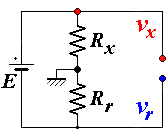
\includegraphics[scale = 1.5]{Partitore di tensione di riferimento nell'ohmetro.png}
\end{figure}

Risolvendo questo semplice problema di elettrotecnica, avremo che $v_x(t)$ e $v_r (t)$ sono esprimibili come:

{
    \Large 
    \begin{equation}
        \begin{cases}
            v_x = E \cdot \frac{R_x}{R_x + R_r} 
            \\
            v_r = - E \cdot \frac{R_r}{R_x + R_r} 
        \end{cases}
    \end{equation}
}

Queste relazioni valgono solo se il circuito è a vuoto, cioè se nei nodi di $v_x$ e $v_r$ non è presente nessun componente. \newline 

Utilizzando il concetto della massa virtuale degli AmpOp e la loro possibilità di isolare due circuiti, 
possiamo aggiungere all'architettura dell'ohmetro un AmpOp in modalità inseguitore. \newline 

Cioè si passa da: 

\begin{figure}[h]
    \centering
    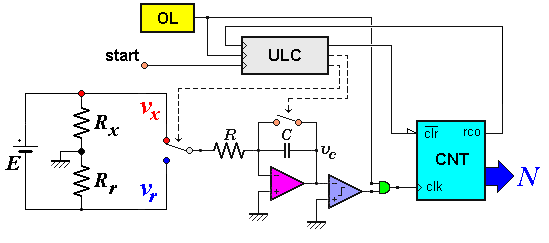
\includegraphics[scale = 1]{Architettura ohmetro.png}
\end{figure}

a questo tipo di architettura: 

\begin{figure}[h]
    \centering
    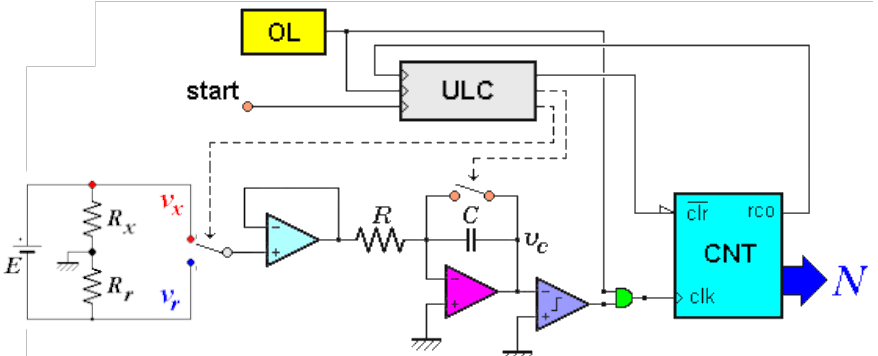
\includegraphics[scale = 2]{Architettura ohmetro reale.png}
\end{figure}

L'AmpOp, in questo caso, in modalità inseguitore, è un buffer inseguitore perchè applica una tensione immediata al resistore R, 
in modo da far circolare una corrente e caricare la capacità C in modo istantaneo. \newline

\newpage 

\section{Caratteristiche metrologiche: risoluzione}
\footnote{Slide della prof | SDME 4 Strumenti numerici indicatori - parte VI | pag 24 \\  
Appunti | 2025-05-20 | pag 1}

Data l'architettura del voltmetro + amperometro: 

\begin{figure}[h]
    \centering
    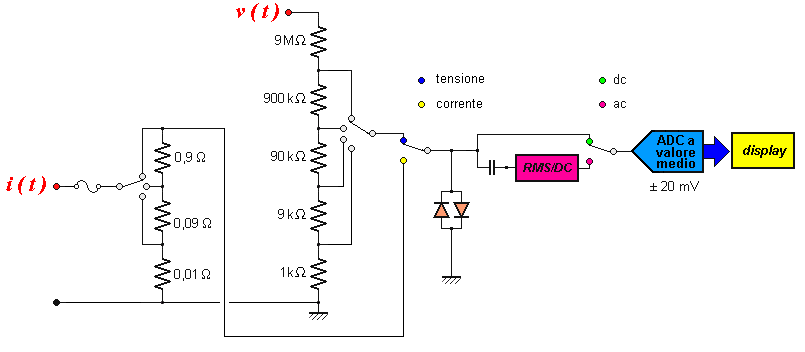
\includegraphics[scale = 1]{Amperometro + Voltmetro.png}
\end{figure}

si vuole analizzare la risoluzione dello strumento, risoluzione che dipende da: 

\begin{itemize}
    \item dalla quantizzazione con cui opera il convertitore AD 
    \item dalla portata selezionata perchè ciò che viene quantizzato è una frazione del misurando 
\end{itemize}

Si utilizza fisicamente lo stesso multimetro per le diverse portate del voltmetro e dell'amperometro. \newline 

Dal punto di vista misuristico, la risoluzione dell'ADC è la stessa per tutte le portate:
ecco perchè l'ADC ha un ruolo fondamentale nella misura in un multimetro. \newline 

La risoluzione dello strumento finale è diversa dalla risoluzione dell'ADC. \newline 


\newpage 

\section{Caratteristiche metrologiche: incertezza}
\footnote{Slide della prof | SDME 4 Strumenti numerici indicatori - parte VI | pag 25 \\  
Appunti | 2025-05-20 | pag 1}

Dato un multimetro, dobbiamo calcolarci la sua incertezza. \newline 

Se è espressa in forma binomiale, data una grandezza g, l'incertezza dello strumento $\Delta g$ equivale a: 

{
    \Large 
    \begin{equation}
        \Delta g 
        = 
        \pm 
        (a \% \text{ lettura } + b \text{ digit })
    \end{equation}
}

\newpage 

\section{Incertezza del multimetro}
\footnote{Slide della prof | SDME 4 Strumenti numerici indicatori - parte VI | pag 26 \\  
Appunti | 2025-05-20 | pag 1}

Data una architettura di un voltmetro, 
i componenti fisici che causano incertezza sono (quelli cerchiati in rosso): 

\begin{figure}[h]
    \centering
    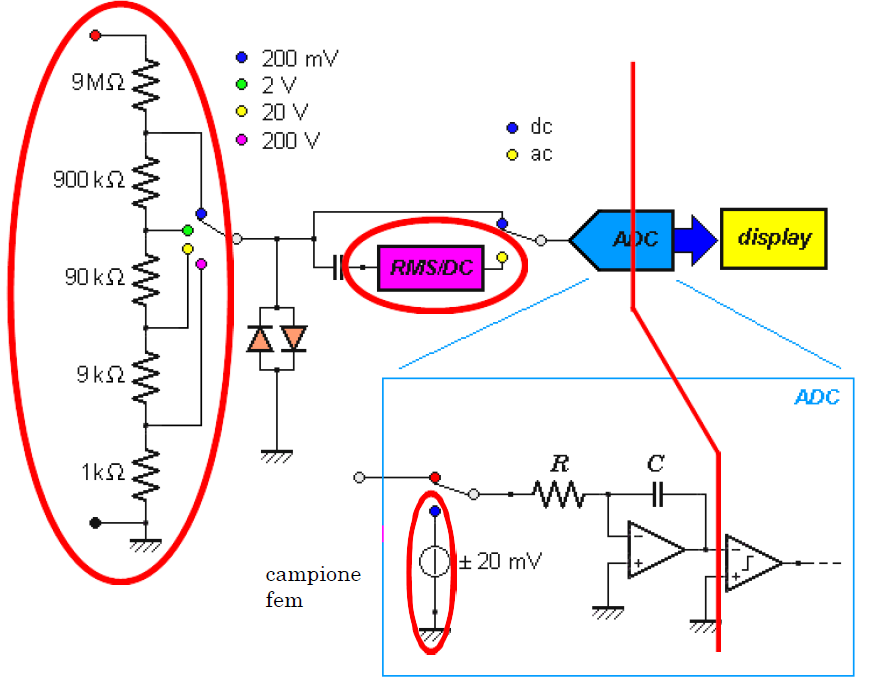
\includegraphics[scale = 1]{Cause di incertezza in un voltmetro.PNG}
\end{figure}

In particolare, gli elementi che causano più incertezza negli strumenti sono i resistori, 
che, anche se sono di precisione e sono costruiti "a regola d'arte" e il loro valore nominale è stabile, 
sono i componenti, in un multimetro, più dipendenti dalla temperatura. \newline 

\newpage 

\subsection{Deriva termica dei resistori: partitore del voltmetro}
\footnote{Slide della prof | SDME 4 Strumenti numerici indicatori - parte VI | pag 27 - 28 \\  
Appunti | 2025-05-20 | pag 1 - 2}

Data la rete resistiva di un voltmetro: 

\begin{figure}[h]
    \centering
    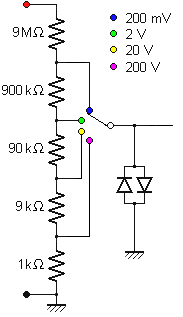
\includegraphics[scale = 1]{Rete resistiva voltmetro.png}
\end{figure}

andiamo a modellare i calcoli in modo che siano due resistori $R_1$ e $R_2$ che l'ADC vedrebbe nel suo nodo di ingresso: 

\begin{figure}[h]
    \centering
    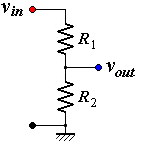
\includegraphics[scale = 2]{Partitore resistivo di due resistori.png}
\end{figure}

Dato un resistore, 
il suo valore di resistenza R può essere modellato con questa relazione lineare: 

{
    \Large 
    \begin{equation}
        R = R_0 [1 + \alpha (\theta - \theta_0)]
    \end{equation}
}

dove:

\begin{itemize} 
    \item $\alpha$ è il TCR (Temperature Coefficient Ratio) che si misura in $[\frac{\Omega}{K}]$ oppure in $[\frac{\Omega}{^{\circ} C}]$, generalmente è maggiore di zero
    \item $\theta_0$ è la temperatura di riferimento con il quale è stato tarato il resistore (generalmente è $25 ^{\circ} C$)
    \item $\theta$ è la temperatura in cui si trova il resistore
    \item $R_0$ è il valore nominale del resistore, cioè il valore con il quale è stato tarato a temperatura $\theta_0$
\end{itemize}


Ritornando al partitore di tensione di $R_1$ e $R_2$, 
dato un semplice esercizio di elettrotecnica, 
possiamo definire la tensione $v_{out}$ come: 

{
    \Large 
    \begin{equation}
        v_{out}
        = 
        v_{in}
        \cdot 
        \frac{R_2}{R_1 + R_2}
    \end{equation}
}

Sostituendo all'equazione di $v_{out}$ i modelli lineari dei due resistori: 

{
    \Large 
    \begin{equation}
        \begin{split}
        v_{out}
        &= 
        v_{in}
        \cdot 
        \frac{R_2}{R_1 + R_2} 
        \\
        &\downarrow
        \\
        v_{out}
        &=
        v_{in}
        \cdot 
        \frac{ R_{20} [1 + \alpha_2 (\theta - \theta_0)]}{R_{10} [1 + \alpha_1 (\theta - \theta_0)] + R_{20} [1 + \alpha_2 (\theta - \theta_0)]}
        \end{split}
    \end{equation}
}

dove: 

\begin{itemize}
    \item $R_{10}$ e $R_{20}$ sono i valori nominali di, rispettivamente, $R_1$ e $R_2$
    \item $\alpha_1$ e $\alpha_2$ sono i TCR di, rispettivamente, $R_1$ e $R_2$
\end{itemize}


Se consideriamo: 

{
    \Large 
    \begin{equation}
        \alpha = \alpha_1 = \alpha_2
    \end{equation}
}

allora, possiamo semplificare i calcoli e facendo qualche passaggio algebrico: 

{
    \Large 
    \begin{equation}
        \begin{split}
        v_{out}
        &=
        v_{in}
        \cdot 
        \frac{ R_{20} [1 + \alpha_2 (\theta - \theta_0)]}{R_{10} [1 + \alpha_1 (\theta - \theta_0)] + R_{20} [1 + \alpha_2 (\theta - \theta_0)]} 
        \\
        &\downarrow
        \\
        v_{out}
        &=
        v_{in}
        \cdot 
        \frac{ R_{20} [1 + \alpha (\theta - \theta_0)]}{R_{10} [1 + \alpha (\theta - \theta_0)] + R_{20} [1 + \alpha (\theta - \theta_0)]} 
        \\
        &=
        v_{in}
        \cdot 
        \frac{ R_{20} [1 + \alpha (\theta - \theta_0)]}{(R_{10} + R_{20}) \cdot [1 + \alpha (\theta - \theta_0)] } 
        \\
        &= 
        v_{in}
        \cdot 
        \frac{R_{20}}{R_{10} + R_{20}}
        \\
        &=
        v_{out_0}
    \end{split}
    \end{equation}
}

Quindi, da questi semplici conti, abbiamo visto che, se tutti i resistori della rete resistiva del voltmetro hanno lo stesso TCR e si trovano alla stessa temperatura:

{
    \Large 
    \begin{equation}
        v_{out}
        = 
        v_{out_0}
    \end{equation}
}

cioè il valore nominale calcolato "carta e penna" del modello teorico è uguale alla tensione che avremo realmente all'ADC. \newline 

Inoltre, si può dire che la temperatura non influisce (o influisce poco) nel risultato di misura, 
e che la misura di tensione è robusta al variare della temperatura. \newline 

\newpage 

\subsection{Deriva termica dei resistori: shunt dell'amperometro}
\footnote{Slide della prof | SDME 4 Strumenti numerici indicatori - parte VI | pag 29 \\  
Appunti | 2025-05-20 | pag 2 | 2025-06-23 Ricevimento | pag 12 - 13} 

Stabilita una portata, possiamo modellizzare il circuito dello stadio di ingresso di un amperometro con un fusibile e un resistore a resistenza fissa R: 

\begin{figure}[h]
    \centering
    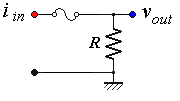
\includegraphics[scale = 2]{Stadio di ingresso amperometro.png}
\end{figure}

Sapendo il modello lineare del resistore: 

{
    \Large 
    \begin{equation}
        R = R_0 [1 + \alpha (\theta - \theta_0)]
    \end{equation}
}

e sapendo che, idealmente, 
nell'amperometro la tensione che va nell'ADC $v_{out_0}$ vale: 

{
    \Large 
    \begin{equation}
        v_{out_0} 
        = 
        i_{in}
        \cdot 
        R_0
    \end{equation}
}


Nella realtà, in uno stadio di ingresso di un amperometro: 

\begin{figure}[h]
    \centering
    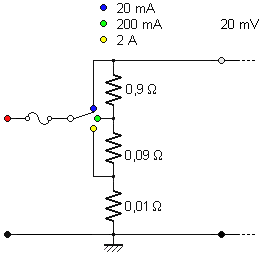
\includegraphics[scale = 1.5]{Stadio di ingresso amperometro A.png}
\end{figure}

Ponendo il modello lineare del resistore R, 
la tensione che va all'ADC reale $v_{out}$ vale: 

{
    \Large 
    \begin{equation}
        \begin{split}
        v_{out}
        &= 
        i_{in}
        \cdot 
        R
        \\
        &= 
        i_{in}
        \cdot 
        R_0 [1 + \alpha (\theta - \theta_0)] 
        \\
        &= 
        v_{out_0}
        \cdot 
        [1 + \alpha (\theta - \theta_0)]
        \end{split}
        \end{equation}
}

L'equazione: 

{
    \Large 
    \begin{equation}
      v_{out}
        =  
        v_{out_0}
        \cdot 
        [1 + \alpha (\theta - \theta_0)]
    \end{equation}
}

dimostra che, purtroppo, a differenza del voltmetro, la misura di $v_{out}$ per l'ADC 
è una misura che dipende dalla temperatura in cui si trovano i resistori all'interno dell'amperometro. \newline 

La misura svolta nello stadio di ingresso di un amperometro non è una misura potenziometrica. \newline 

Per misura potenziometrica si intende che tutta la potenza di ingresso ricade su tutta la rete resistiva. \newline 

Nel volmentro ciò accade, nell'amperometro no perchè, a meno che non si scelga la portata a 20 mA, 
tutta la potenza di ingresso non ricade su tutta la rete resistiva, solo una parte. \newline 

\newpage

\section{Resistori di precisione}
\footnote{Slide della prof | SDME 4 Strumenti numerici indicatori - parte VI | pag 30 \\  
Appunti | 2025-05-20 | pag 2}

Per precisione si intende che, nelle misure ripetute, la deviazione standard è minore, 
cioè la differenza tra le varie misure ripetute e il valore centrale è piccola. \newline 

Un resistore di precisione utilizzato tipicamente nei voltmetri è quello in filo metallico avvolto: 

\begin{figure}[h]
    \centering
    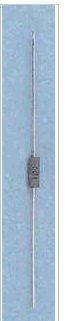
\includegraphics[scale = 1]{Filo metallico avvolto resistore.png}
\end{figure}

Le caratteristiche di un resistore di precisione in filo metallico avvolto sono le seguenti: 

\begin{itemize}
    \item tolleranza resistenza $\pm 50$ ppm 
    \item coefficiente di temperatura $\pm 10 $ ppm / $^{\circ} C$ 
    \item potenza dissipata 0.25 W a 125 $^{\circ} C$
\end{itemize}

In commercio, i resistori di precisione in filo metallico presentano un coefficiente di temperatura $\pm 10 $ ppm / $^{\circ} C$ , 
ma, sono disponibili nel mercato altri resistori di precisione in filo metallico con TCR fino a $\pm 1 $ ppm / $^{\circ} C$ . \newline 

Un resistore di precisione utilizzato tipicamente nel convertitore i-v per amperometro e che viene anche utilizzato come resistore di riferimento per l'ohmmetro 
è il resistore di precisione in metallo massiccio: 

\begin{figure}[h]
    \centering
    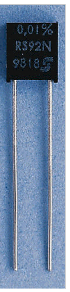
\includegraphics[scale = 1]{Resistore di preicisone in metallo massiccio.png}
\end{figure}

Le caratteristiche di un resistore di precisione in metallo massiccio sono le seguenti: 

\begin{itemize}
    \item tolleranza resistenza $\pm 100$ ppm 
    \item coefficiente di temperatura $\pm 5 $ ppm / $^{\circ} C$ con accordo fino a $\pm 1 $ ppm / $^{\circ} C$ 
    \item potenza dissipata 0.6 W a 70 $^{\circ} C$
\end{itemize}

Quindi, negli ohmmetri e nei convertitori i-v si accetta una tolleranza di resistenza maggiore rispetto ai resistori nei voltmetri. \newline 

Siccome abbiamo visto nelle scorse sezioni che la corrente di ingresso allo strumento è calcolata in base alla tensione ai capi dei resistori 
e, quest'ultima, dipende dalla differenza tra la temperatura del resistore e la temperatura con cui è stato tarato, 
allora è richiesto un coefficiente di temperatura minore rispetto ai resistori nei voltmetri, nonostante si abbia una tolleranza resistiva maggiore. \newline 

\newpage 